\documentclass[10pt,a4paper]{article}
\usepackage[T1]{fontenc}
\usepackage[utf8]{inputenc}
\usepackage{lmodern}
\usepackage{microtype}
\usepackage[a4paper,top=16mm,bottom=16mm,left=17mm,right=17mm,headheight=9mm,footskip=9mm]{geometry}
\usepackage{xcolor}
\usepackage{graphicx}
\usepackage{booktabs}
\usepackage{tabularx}
\usepackage{array}
\usepackage{enumitem}
\usepackage{tikz}
\usetikzlibrary{arrows.meta,positioning,shapes.geometric,calc,fit}
\usepackage[most]{tcolorbox}
\usepackage{fancyhdr}
\usepackage{lastpage}
\usepackage{hyperref}
\usepackage{pdflscape}
\usepackage{ragged2e}
\usepackage{seqsplit}
\usepackage{titlesec}
\usepackage{amsmath}

\definecolor{Navy}{HTML}{102A43}
\definecolor{Blue}{HTML}{1666A8}
\definecolor{Cyan}{HTML}{2D9CDB}
\definecolor{Teal}{HTML}{168C86}
\definecolor{Green}{HTML}{23856D}
\definecolor{Orange}{HTML}{E56B2F}
\definecolor{Amber}{HTML}{D99A1D}
\definecolor{Red}{HTML}{B54747}
\definecolor{Ink}{HTML}{243B53}
\definecolor{Muted}{HTML}{627D98}
\definecolor{Line}{HTML}{D9E2EC}
\definecolor{Panel}{HTML}{F4F7FA}
\definecolor{PaleBlue}{HTML}{EAF3FA}
\definecolor{PaleOrange}{HTML}{FFF1E8}
\definecolor{PaleGreen}{HTML}{EAF7F2}
\definecolor{PaleRed}{HTML}{FAECEC}

\hypersetup{colorlinks=true,linkcolor=Blue,urlcolor=Blue,pdftitle={Epoxy/Amine Compound Funnel --- Phase-0 Implementation and Readiness Review},pdfauthor={Amphora Engineering}}
\setlength{\parindent}{0pt}
\setlength{\parskip}{3.5pt}
\setlist[itemize]{leftmargin=4.2mm,itemsep=1.3pt,topsep=2pt}
\setlist[enumerate]{leftmargin=5mm,itemsep=1.3pt,topsep=2pt}
\renewcommand{\arraystretch}{1.18}
\pagestyle{fancy}
\fancyhf{}
\fancyhead[L]{\sffamily\fontsize{7.2}{8}\selectfont\color{Muted} AMPHORA / CONTROLLED IMPLEMENTATION REVIEW}
\fancyhead[R]{\sffamily\fontsize{7.2}{8}\selectfont\color{Muted} 19 JUL 2026 / AUDIT\_ONLY}
\fancyfoot[L]{\sffamily\fontsize{7}{8}\selectfont\color{Muted} Unmade digital proposals; no safety, procurement, synthesis, qualification, or execution authority}
\fancyfoot[R]{\sffamily\fontsize{7}{8}\selectfont\color{Muted} \thepage\ / \pageref{LastPage}}
\renewcommand{\headrulewidth}{0.3pt}
\renewcommand{\footrulewidth}{0pt}
\titleformat{\section}{\sffamily\bfseries\Large\color{Navy}}{}{0pt}{}[\vspace{1mm}\color{Cyan}\rule{18mm}{1.2pt}]
\titleformat{\subsection}{\sffamily\bfseries\normalsize\color{Navy}}{}{0pt}{}
\newcommand{\PageTitle}[2]{%
  {\sffamily\fontsize{7.5}{9}\selectfont\bfseries\color{Cyan}\MakeUppercase{#1}}\\[-1pt]
  {\sffamily\fontsize{20}{22}\selectfont\bfseries\color{Navy}#2}\par\vspace{3mm}}
\newcommand{\eyebrow}[1]{{\sffamily\fontsize{7}{8}\selectfont\bfseries\color{Cyan}\MakeUppercase{#1}}}
\newcommand{\metric}[3]{%
  \begin{tcolorbox}[enhanced,boxrule=0pt,colback=#3,arc=2mm,left=2.5mm,right=2.5mm,top=2mm,bottom=2mm]
  {\sffamily\fontsize{17}{18}\selectfont\bfseries\color{Navy}#1}\par
  {\sffamily\fontsize{7.2}{8.4}\selectfont\color{Muted}#2}
  \end{tcolorbox}}
\newcommand{\callout}[2]{%
  \begin{tcolorbox}[enhanced,breakable,colback=Panel,colframe=Line,boxrule=.45pt,arc=2mm,left=3mm,right=3mm,top=2.5mm,bottom=2.5mm]
  {\sffamily\bfseries\color{Navy}#1}\par #2
  \end{tcolorbox}}
\newcommand{\good}{\textcolor{Green}{\bfseries GOOD}}
\newcommand{\bad}{\textcolor{Red}{\bfseries BAD / BLOCKED}}
\newcommand{\lefttodo}{\textcolor{Amber}{\bfseries LEFT}}
\newcommand{\phasezero}{\textcolor{Green}{\bfseries PHASE 0}}
\newcommand{\prephase}{\textcolor{Amber}{\bfseries PRE}}
\newcommand{\code}[1]{{\ttfamily\fontsize{7.2}{8.4}\selectfont\detokenize{#1}}}
\newcolumntype{Y}{>{\RaggedRight\arraybackslash}X}
\newcolumntype{C}[1]{>{\centering\arraybackslash}p{#1}}

\begin{document}

% PAGE 1 — COVER
\thispagestyle{empty}

\begin{tikzpicture}[remember picture,overlay]
  \fill[Navy] (current page.south west) rectangle (current page.north east);
  \fill[Blue,opacity=.50] ($(current page.north east)+(-18mm,-26mm)$) circle (38mm);
  \fill[Cyan,opacity=.24] ($(current page.north east)+(-52mm,-6mm)$) circle (22mm);
  \fill[Orange,opacity=.80] ($(current page.south west)+(20mm,26mm)$) circle (4mm);
  \draw[Cyan,line width=1.4pt,opacity=.85]
    ($(current page.south west)+(16mm,64mm)$) -- ++(22mm,0) -- ++(12mm,18mm) -- ++(22mm,0);
  \draw[Orange,line width=1.4pt,opacity=.85]
    ($(current page.south west)+(38mm,64mm)$) -- ++(12mm,-18mm) -- ++(22mm,0);
\end{tikzpicture}
\vspace*{18mm}
{\sffamily\fontsize{9}{11}\selectfont\bfseries\color{Cyan} AMPHORA / IMPLEMENTATION \& READINESS REVIEW}\par
\vspace{20mm}
{\sffamily\fontsize{34}{37}\selectfont\bfseries\color{white} Epoxy / Amine\\Compound Funnel}\par
\vspace{5mm}
{\sffamily\fontsize{17}{21}\selectfont\color{white!78} Non-ranking digital proposals to\\CRO feasibility-review packets}\par
\vspace{14mm}
\begin{tcolorbox}[width=136mm,colback=white!7,colframe=white!22,boxrule=.6pt,arc=2mm,left=5mm,right=5mm,top=4mm,bottom=4mm]
{\sffamily\fontsize{10}{13}\selectfont\color{white}
Implementation snapshot \textbf{19 July 2026} \quad\textcolor{Cyan}{/}\quad Authority \textbf{AUDIT\_ONLY}\\[2mm]
Current portfolio \textbf{8 Phase 0 / 21 pre-Phase-0} \quad\textcolor{Cyan}{/}\quad Target \textbf{12 / 17}}
\end{tcolorbox}
\vfill
{\sffamily\fontsize{9}{12}\selectfont\color{white!70}
Detailed design, module-by-module status, evidence gaps, acceptance record, throughput, and 20 final observed compound audit cards.}
\vspace{12mm}
{\sffamily\fontsize{7.5}{9}\selectfont\bfseries\color{Orange} LOCKED\_INTERNAL \quad / \quad NO RANKING \quad / \quad NO LAB EXECUTION}
\newpage

% PAGE 2 — EXECUTIVE
\PageTitle{01 / Executive decision}{The funnel is implemented; promotion is not yet earned}
\begin{minipage}[t]{.235\linewidth}\metric{8 / 21}{Phase 0 / pre-Phase-0 today}{PaleBlue}\end{minipage}\hfill
\begin{minipage}[t]{.235\linewidth}\metric{210}{workspace tests passing}{PaleGreen}\end{minipage}\hfill
\begin{minipage}[t]{.235\linewidth}\metric{13 / 29}{locked diagnostics passing}{PaleOrange}\end{minipage}\hfill
\begin{minipage}[t]{.235\linewidth}\metric{0}{scientific ranks emitted}{PaleRed}\end{minipage}

\vspace{2mm}
\callout{Decision in one sentence}{The software boundaries, locked manifests, typed property-to-formulation chain, signed non-executable CRO packet, sparse Phase-0 runtime grants, ORD acquisition verifier, rights workflow, and non-ranking campaign CLI now exist and pass the ordinary workspace suite; the four module movements are correctly withheld because ORD objects, the provenance-built RDKit runtime, rights receipts, independent signatures, locked campaign evidence, and the 96-attack/32-control review have not been supplied.}

\begin{minipage}[t]{.485\linewidth}
\subsection*{What is genuinely good}
\begin{itemize}
  \item Fail-closed authority is intact: every observed envelope has \code{usable_by_optimizer:false}; no objective or rank is emitted.
  \item Exact typed handoffs prevent candidate injection of molecular weight, EEW, AHEW, group counts, or authoritative density.
  \item The v4 catalog is parent-bound to immutable v3 and declares all 550 ORD LFS objects and 1,181,061,030 bytes.
  \item Twenty audit probes traverse 12 controls twice with identical result hashes.
  \item Existing data and global audits pass; v3 retains 738,149 normalized rows and 42,158 explicit rejections.
\end{itemize}
\end{minipage}\hfill
\begin{minipage}[t]{.485\linewidth}
\subsection*{What is not good enough}
\begin{itemize}
  \item v4 has one acquisition unit pending and zero acquired ORD objects; a catalog of pointers is not the reaction corpus.
  \item The exact C++ RDKit build manifest and library hashes are not installed; feature tests fail closed at the build boundary.
  \item Rights verification has no active non-development reviewer identity.
  \item No 24-structure campaign cohort, 12 verified pair packets, or campaign KPI denominator exists yet.
  \item The requested sealed independent attacks and 32 valid controls have not been received or executed.
\end{itemize}
\end{minipage}

\vspace{2mm}
\begin{tcolorbox}[colback=Navy,colframe=Navy,arc=2mm,left=4mm,right=4mm,top=3mm,bottom=3mm]
{\color{white}\sffamily\bfseries Truth boundary.} {\color{white!82}The 20 structures at the end are pre-campaign audit probes, not ORD-generated campaign outputs. ``Final'' means final observed card at this implementation snapshot. It does not mean synthesized, safe, available, novel, qualified, or selected.}
\end{tcolorbox}
\newpage

% PAGE 3 — ARCHITECTURE
\PageTitle{02 / Overall design}{A hash-bound funnel with authority separated from computation}
\begin{center}
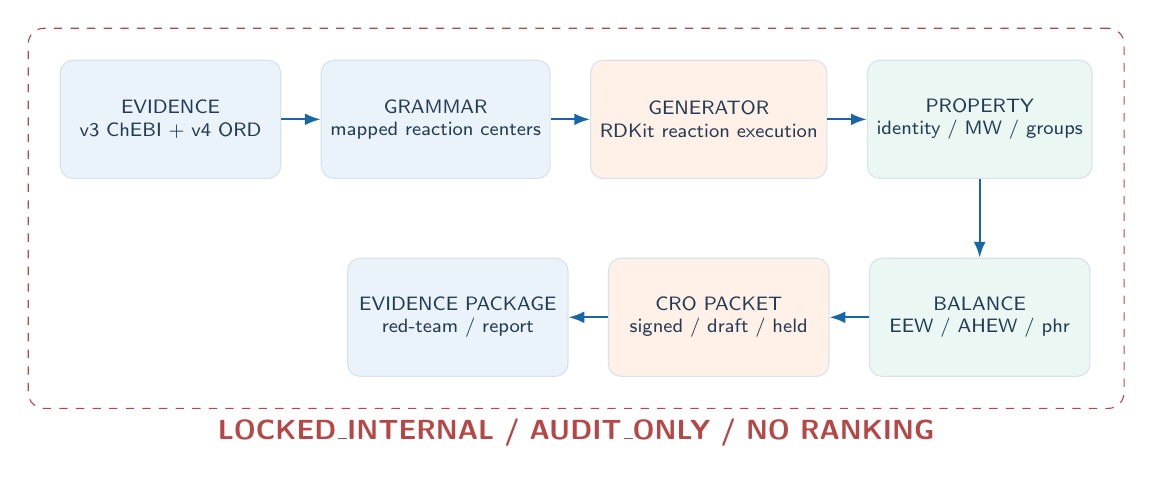
\begin{tikzpicture}[node distance=7mm and 5mm, every node/.style={font=\sffamily\fontsize{7.1}{8}\selectfont,align=center}, box/.style={rounded corners=1.6mm,minimum width=28mm,minimum height=15mm,draw=Line,fill=white,text=Ink}, arr/.style={-{Latex[length=2mm]},line width=.8pt,draw=Blue}]
\node[box,fill=PaleBlue] (e) {EVIDENCE\\v3 ChEBI + v4 ORD};
\node[box,right=of e,fill=PaleBlue] (g) {GRAMMAR\\mapped reaction centers};
\node[box,right=of g,fill=PaleOrange] (gen) {GENERATOR\\RDKit reaction execution};
\node[box,right=of gen,fill=PaleGreen] (prop) {PROPERTY\\identity / MW / groups};
\node[box,below=10mm of prop,fill=PaleGreen] (bal) {BALANCE\\EEW / AHEW / phr};
\node[box,left=of bal,fill=PaleOrange] (cro) {CRO PACKET\\signed / draft / held};
\node[box,left=of cro,fill=PaleBlue] (pkg) {EVIDENCE PACKAGE\\red-team / report};
\draw[arr] (e)--(g); \draw[arr] (g)--(gen); \draw[arr] (gen)--(prop);
\draw[arr] (prop)--(bal); \draw[arr] (bal)--(cro); \draw[arr] (cro)--(pkg);
\node[draw=Red,dashed,rounded corners=2mm,fit=(e)(g)(gen)(prop)(bal)(cro)(pkg),inner sep=4mm,label={[font=\sffamily\bfseries\color{Red}]below:LOCKED\_INTERNAL / AUDIT\_ONLY / NO RANKING}] {};
\end{tikzpicture}
\end{center}

\begin{minipage}[t]{.485\linewidth}
\subsection*{Scientific data plane}
\begin{enumerate}
  \item Acquire and verify complete snapshots; normalize without erasing rejects.
  \item Split reaction, canonical-family, and scaffold components before extracting grammar.
  \item Execute only host-authorized reaction SMARTS on the exact backend.
  \item Recompute identity and molecular facts from the resulting graph.
  \item Select cohorts by canonical hash within role/scaffold strata---never by predicted performance.
  \item Compute theoretical equivalent balance and bind draft CRO packets to candidate and formula hashes.
\end{enumerate}
\end{minipage}\hfill
\begin{minipage}[t]{.485\linewidth}
\subsection*{Authority plane}
\begin{enumerate}
  \item Rights, evaluation, and review use three distinct authorized signers.
  \item \code{EngineEvidenceContextV3} activates sparse module-specific grants; unrelated novelty or Process-QC grants are not prerequisites.
  \item Each grant binds movement, evaluation, review, rights overlay, benchmark, model/grammar, inputs, and claim locks.
  \item Every CRO packet is \code{DRAFT_FOR_CRO_FEASIBILITY_REVIEW}, signed, non-executable, and held for material, chemist/EHS, and CRO acceptance.
  \item Movement is atomic and module-specific. Failed science remains visible and cannot be converted into authority.
\end{enumerate}
\end{minipage}

\callout{The central design choice}{Computation and authority are deliberately orthogonal. A module can calculate a diagnostic value while remaining unable to rank, recommend procurement, authorize synthesis, claim safety, or release a formulation. Conversely, a signature cannot replace missing chemistry, data, denominators, or negative results.}

\begin{tabularx}{\linewidth}{@{}p{31mm}Y Y@{}}
\toprule
\textbf{Boundary} & \textbf{Accepted} & \textbf{Rejected / quarantined} \\
\midrule
Grammar & Signed host artifact bound to ORD IDs, family, SMARTS, constraints, and hashes & Candidate-supplied SMARTS, source IDs, grammar, or substituted artifact \\
Molecule facts & Exact host RDKit graph result and its hash & Candidate MW, formula, EEW/AHEW, group count, identity override \\
Protocol authority & Locked protocol reference for numeric thresholds & Packet-authored performance threshold or implied execution \\
\bottomrule
\end{tabularx}
\newpage

% PAGE 4 — DATA
\PageTitle{03 / Evidence and trust}{Immutable catalogs are ready; the external evidence is not}
\begin{tabularx}{\linewidth}{@{}p{24mm}p{24mm}p{32mm}Y@{}}
\toprule
\textbf{Layer} & \textbf{Audit state} & \textbf{Measured content} & \textbf{Interpretation} \\
\midrule
feedback/v3 & \textcolor{Green}{PASS} & 6/6 units; 738,149 rows; 42,158 rejects & Existing corpus is immutable. ChEBI release 252 remains available, but property rights receipt is absent. \\
feedback/v4 & \textcolor{Green}{PASS catalog} / \textcolor{Amber}{PENDING data} & 1 unit declared; 0 acquired; 550 ORD objects; 1.181 GB & Parent hash binds v3. Every official LFS OID, byte size, path, and expected raw SHA is declared. \\
RDKit C++ & \textcolor{Red}{ABSENT} & Release 2026.03.2, commit \code{42fe8c...}, source SHA pinned & Reproducible container recipe exists; build and library receipts do not. Feature compilation refuses missing paths. \\
Rights identities & \textcolor{Red}{ABSENT} & request / offline-sign / import / verify flow implemented & Trust store has no active independent rights reviewer; no repository private key is accepted. \\
\bottomrule
\end{tabularx}

\vspace{3mm}
\begin{minipage}[t]{.485\linewidth}
\subsection*{ORD\_GIT\_LFS\_TREE hard gates}
\begin{itemize}
  \item exact official repository and Git commit \code{ddb0d257...};
  \item exact 550 \code{.pb.gz} path set---no unexpected or missing object;
  \item pointer OID equals retrieved raw SHA-256 and declared size;
  \item no symlink, unresolved pointer, partial retrieval, corrupt object, or companion-file substitution;
  \item immutable content-addressed installation plus signed acquisition receipt;
  \item re-audit of the complete installed set before normalization.
\end{itemize}
\end{minipage}\hfill
\begin{minipage}[t]{.485\linewidth}
\subsection*{Leakage-safe grammar policy}
\begin{itemize}
  \item Parse only explicit, single-component, atom-mapped reactants and products with provenance.
  \item Derive a well-defined reaction center or reject with a reason.
  \item Partition connected reaction identity, canonical compound family, and scaffold components before extraction.
  \item Keep ORD-derived grammar in the CC-BY-SA-4.0 evidence layer; do not copy it into MIT source.
  \item Export attribution and share-alike metadata with every derived grammar and CRO evidence bundle.
\end{itemize}
\end{minipage}

\callout{Observed failure is correct}{\code{compound campaign run --locked ...} stops at ``complete ORD Git LFS snapshot has not been acquired.'' The RDKit feature build stops at missing \code{RDKIT_INCLUDE_DIR}. Both are desired fail-closed behavior; neither is campaign success.}

\subsection*{Trust ceremony still required}
Day zero must register and prove possession of three distinct, non-revoked, non-development Ed25519 identities: rights reviewer, evaluator, and independent reviewer. Cross-role reuse, stale receipts, same-signer review, wrong snapshot, wrong module, stripped exclusions, or repository-local private material is rejected.

\begin{tcolorbox}[colback=PaleOrange,colframe=Orange!45,boxrule=.5pt,arc=2mm]
\textbf{Licensing posture.} ORD snapshot and derived grammar are treated as CC-BY-SA-4.0 evidence. ChEBI release 252 is treated as CC-BY-4.0 input. This is an implementation control, not a legal opinion; the signed rights reviewer remains the authority required by the movement gate.
\end{tcolorbox}
\newpage

% PAGE 5 — ALL MODULES
\PageTitle{04 / Portfolio register}{Every native module and its current phase}
{\sffamily\fontsize{7.2}{8.5}\selectfont\color{Muted}Measured by \code{portfolio phase0 status --all}. Eight modules have signed Phase-0 movements; 21 remain pre-Phase-0. All 29 are confined to non-ranking authority.}\par
\vspace{3mm}
\begin{minipage}[t]{.492\linewidth}
\begin{tcolorbox}[colback=white,colframe=Line,boxrule=.5pt,arc=1.5mm,left=2mm,right=2mm,top=2mm,bottom=2mm]
\begin{tabularx}{\linewidth}{@{}Y C{10mm} C{20mm}@{}}
\toprule \textbf{Module} & \textbf{P} & \textbf{Primary signal} \\
\midrule
barrier-corrosion-score & \prephase & S/R/E \\
candidate-contract & \textcolor{Green}{\bfseries P0} & complete \\
cro-protocol-packager & \prephase & E \\
cure-potlife-gate & \prephase & R/E \\
design-rule-score & \prephase & S/R/E \\
envelope-gates & \prephase & E \\
evidence-intake-validator & \textcolor{Green}{\bfseries P0} & complete \\
formulation-arithmetic & \prephase & E \\
formulation-universe & \prephase & E \\
ingredient-library & \prephase & S/R/E \\
ip-fto-guard & \prephase & R/E \\
known-answer-benchmarks & \prephase & S/R/E \\
model-card-authority & \textcolor{Green}{\bfseries P0} & complete \\
molecule-design-gate & \textcolor{Green}{\bfseries P0} & complete \\
molecule-generator & \prephase & ORD/R/E \\
\bottomrule
\end{tabularx}
\end{tcolorbox}
\end{minipage}\hfill
\begin{minipage}[t]{.492\linewidth}
\begin{tcolorbox}[colback=white,colframe=Line,boxrule=.5pt,arc=1.5mm,left=2mm,right=2mm,top=2mm,bottom=2mm]
\begin{tabularx}{\linewidth}{@{}Y C{10mm} C{20mm}@{}}
\toprule \textbf{Module} & \textbf{P} & \textbf{Primary signal} \\
\midrule
molecule-novelty & \prephase & S/R/D/E \\
molecule-property & \prephase & S/R/E \\
molecule-role-ranker & \prephase & R/E \\
optimizer-orchestrator & \prephase & E \\
process-qc-twin & \prephase & R auth \\
public-corrosion-benchmark & \prephase & S/R/E \\
redteam-audit & \textcolor{Green}{\bfseries P0} & complete \\
report-packager & \textcolor{Green}{\bfseries P0} & complete \\
run-provenance & \textcolor{Green}{\bfseries P0} & complete \\
solvency-score & \prephase & S/R/E \\
source-ledger & \textcolor{Green}{\bfseries P0} & complete \\
sourceability-ehs & \prephase & R/E \\
tolerance-robustness & \prephase & S/R/E \\
viscosity-score & \prephase & S/R/E \\
\multicolumn{3}{l}{\textbf{Portfolio: 8 Phase 0 / 21 pre-Phase-0}} \\
\bottomrule
\end{tabularx}
\end{tcolorbox}
\end{minipage}

{\sffamily\fontsize{6.7}{7.7}\selectfont\color{Muted}Signal key: S source lock; R rights; D required data; E external evaluation; auth cryptographic authorization.}

\vspace{3mm}
\begin{tabularx}{\linewidth}{@{}p{36mm}C{17mm}C{20mm}Y@{}}
\toprule
\textbf{Promotion target} & \textbf{Phase} & \textbf{Locked diagnostic} & \textbf{Status interpretation} \\
\midrule
molecule-property & PRE & FAIL / AUDIT & Implementation present; exact backend, locked ontology, rights overlay, 300-structure benchmark, evaluator and reviewer absent. \\
molecule-generator & PRE & FAIL / ROADMAP & Authorized reaction execution present; ORD objects, extracted grammar, 24-structure cohort, rights and review absent. \\
formulation-arithmetic & PRE & PASS / COMPLETE & Deterministic legacy diagnostic passes; typed host-facts balance is implemented, but external evaluation and movement are absent. \\
cro-protocol-packager & PRE & PASS / COMPLETE & Deterministic packet diagnostic passes; V2 signed draft/holds implemented, but candidate-bound 12-packet campaign and movement are absent. \\
\bottomrule
\end{tabularx}

\callout{Why 12 / 17 was not written into the ledger}{The plan explicitly forbids substituting synthetic records or weakening gates. A passing implementation test is not an external evaluation signature; a report-only structure is not an ORD-generated proposal; and a deterministic CRO fixture is not one of the required 12 candidate-bound feasibility packets. The correct portfolio therefore remains 8 / 21.}
\newpage

% PAGE 6 — PROPERTY & GENERATOR
\PageTitle{05 / Module deep dive I}{Molecule property and molecule generator}
\begin{minipage}[t]{.488\linewidth}
\begin{tcolorbox}[height=160mm,colback=PaleBlue,colframe=Blue!35,boxrule=.6pt,arc=2mm,left=3mm,right=3mm,top=3mm,bottom=3mm]
\eyebrow{01 / amphora-molecule-property}\par
{\sffamily\Large\bfseries\color{Navy}Graph facts, not guessed descriptors}\par
\textbf{Current status:} \prephase\quad \textbf{Diagnostic:} FAIL / AUDIT

\textbf{Implemented}
\begin{itemize}
  \item Exact-backend boundary for canonical isomeric identity, formula, molecular weight, fragments, stereochemistry, oxirane count, reactive amine-H count, and scaffold.
  \item Backend version and ontology version are carried in \code{MoleculeFactsV1}; mismatches fail typed downstream arithmetic.
  \item EEW and AHEW derive only as
  \[\begin{gathered}\mathrm{EEW}=M/n_{oxirane},\\[-1mm]\mathrm{AHEW}=M/n_{amine-H}.\end{gathered}\]
  Zero groups abstain; nonfinite, negative, wildcard, polymer, invalid-valence, and multicomponent cases are rejected or quarantined.
\end{itemize}
\good\ Exact graph-derived facts are structurally separated from candidate claims. Unit and hash provenance are retained.

\bad\ No provenance-built C++ runtime receipt is installed. The required 300-structure locked benchmark and ChEBI rights receipt do not exist.

\lefttodo\ Build the pinned runtime; sign ChEBI rights; run identity/stereo/fragment/invalid/epoxy/amine controls; report formula agreement, mass error distribution, confusion matrix, abstentions, numerator, denominator, rejects, and negative results; obtain evaluator and reviewer signatures.
\end{tcolorbox}
\end{minipage}\hfill
\begin{minipage}[t]{.488\linewidth}
\begin{tcolorbox}[height=160mm,colback=PaleOrange,colframe=Orange!38,boxrule=.6pt,arc=2mm,left=3mm,right=3mm,top=3mm,bottom=3mm]
\eyebrow{02 / amphora-molecule-generator}\par
{\sffamily\Large\bfseries\color{Navy}Authorized reactions with exact lineage}\par
\textbf{Current status:} \prephase\quad \textbf{Diagnostic:} FAIL / ROADMAP

\textbf{Implemented}
\begin{itemize}
  \item Reaction grammar now carries family, reaction SMARTS, ORD source reaction/dataset IDs, applicability constraints, and a stable artifact hash.
  \item Candidate JSON cannot provide or replace grammar. \code{EngineEvidenceContextV3} grants generator access independently of novelty and Process-QC.
  \item The RDKit C++ bridge parses and runs chemical reactions, sanitizes outputs, rejects multi-component products, sorts unique products, and binds parent, seed, grammar, template, source IDs, role, facts, and scaffold.
  \item Without a verified runtime grant, behavior remains \code{QUARANTINED_NO_STRUCTURE_CHANGE}.
\end{itemize}
\good\ The former ID-only mutation path has an authorized structure-changing replacement, with deterministic duplicate and applicability accounting.

\bad\ There is no acquired ORD object set, parsed reaction corpus, extracted held-out grammar, runtime grant, or generated cohort. The 24/8/8/6 thresholds are therefore unmet.

\lefttodo\ Acquire all 550 objects; parse and record exclusions; build leakage-safe components; extract/share-alike grammar; generate at most 96 attempts; retain every duplicate and applicability rejection; meet thresholds without synthetic substitutions; obtain independent replay.
\end{tcolorbox}
\end{minipage}

\vspace{4mm}
\begin{tcolorbox}[colback=Navy,colframe=Navy,arc=2mm,left=4mm,right=4mm,top=3mm,bottom=3mm]
{\color{white}\textbf{Important distinction.}} {\color{white!82}Python RDKit 2026.03.2 was used only to draw the structures in this report and to reject unparseable illustration input. It did not create host-authoritative campaign facts. The campaign requires the separately pinned C++ build, commit, flags, compiler/dependency manifest, and library hashes.}
\end{tcolorbox}
\newpage

% PAGE 7 — BALANCE & CRO
\PageTitle{06 / Module deep dive II}{Equivalent balance and CRO feasibility packaging}
\begin{minipage}[t]{.488\linewidth}
\begin{tcolorbox}[height=151mm,colback=PaleGreen,colframe=Green!35,boxrule=.6pt,arc=2mm,left=3mm,right=3mm,top=3mm,bottom=3mm]
\eyebrow{03 / amphora-formulation-arithmetic}\par
{\sffamily\Large\bfseries\color{Navy}Typed theoretical stoichiometry}\par
\textbf{Current status:} \prephase\quad \textbf{Locked diagnostic:} PASS / COMPLETE

\textbf{Implemented contract: \code{EquivalentBalanceV1}}
\begin{itemize}
  \item Accepts only two host-derived \code{MoleculeFactsV1} values and their stable hashes.
  \item Requires exact backend and ontology, an epoxide-bearing resin, and reactive-amine-H hardener.
  \item Computes resin/hardener mass, EEW, AHEW, epoxide equivalents, amine-H equivalents, hardener phr, equivalent ratio, total mass, and unit provenance.
  \item Persists \code{candidate_property_override_accepted:false}, \code{ranking_eligible:false}, and \code{AUDIT_ONLY}.
\end{itemize}
For resin mass $m_r$ and target ratio $r$:
\[\begin{aligned}n_e&=m_r/\mathrm{EEW}, & m_h&=n_e\,\mathrm{AHEW}\,r,\\[-1mm]
\mathrm{phr}&=100m_h/m_r.&&\end{aligned}\]
\good\ Candidate MW, EEW, AHEW, and group-count injection has no typed entry point. Revalidation recomputes the full record.

\bad\ A deterministic fixture pass is not 12 real pair calculations. No campaign facts exist, so no authoritative EEW/AHEW pair can be emitted.

\lefttodo\ Run 12 deterministic hash-selected pairs after the generated cohort passes; retain all zero-group, unit, hash, nonfinite, and inversion failures; sign evaluation and replay.
\end{tcolorbox}
\end{minipage}\hfill
\begin{minipage}[t]{.488\linewidth}
\begin{tcolorbox}[height=151mm,colback=PaleOrange,colframe=Orange!35,boxrule=.6pt,arc=2mm,left=3mm,right=3mm,top=3mm,bottom=3mm]
\eyebrow{04 / amphora-cro-protocol-packager}\par
{\sffamily\Large\bfseries\color{Navy}A signed draft that cannot execute}\par
\textbf{Current status:} \prephase\quad \textbf{Locked diagnostic:} PASS / COMPLETE

\textbf{Implemented contract: \code{CroProtocolPackageV2}}
\begin{itemize}
  \item Binds candidate JSON/hash, formula hash, and exact \code{EquivalentBalanceV1}.
  \item Requires blinding, custody chain, controls, required outputs, unresolved material/safety fields, chemist/EHS hold, and CRO-acceptance hold.
  \item Status is exactly \code{DRAFT_FOR_CRO_FEASIBILITY_REVIEW}; \code{execution_authorized:false}.
  \item Eight mandatory locks prevent synthesis, safety, performance, qualification, procurement, release, ranking, and execution claims.
  \item Numeric power/decision thresholds appear only through a separately locked protocol reference.
  \item Packet ID and Ed25519 signature are verified; any mutation invalidates the package.
\end{itemize}
\good\ The packet is candidate-bound, formula-bound, signable, byte-stable, and explicitly non-executable.

\bad\ The 12 required campaign packets do not exist. The current locked diagnostic uses controlled fixtures and cannot imply CRO acceptance or results.

\lefttodo\ Create 12 packets only after typed balances exist; verify clean byte replay, signer identity, custody/controls/holds, and prohibited-claim scan; package CC-BY-SA attribution; obtain evaluation and independent review.
\end{tcolorbox}
\end{minipage}

\vspace{4mm}
\callout{No laboratory hand-wave}{A feasibility packet is a structured question for a CRO, not an instruction to execute and not evidence of feasibility. Material availability, chemical review, EHS review, CRO acceptance, detailed locked protocol, synthesis, and testing all remain outside this milestone.}
\newpage

% PAGE 8 — CAMPAIGN / ACCEPTANCE / THROUGHPUT
\PageTitle{07 / Completion path}{What remains, red-team acceptance, and measured rate}
\begin{minipage}[t]{.48\linewidth}
\subsection*{Locked completion sequence}
\begin{enumerate}
  \item Install complete ORD objects and signed rights overlay; build exact RDKit C++ and its manifest.
  \item Benchmark property on $\geq300$ structures and extract leakage-safe reaction grammar.
  \item Generate $\geq24$ unique valid structures: $\geq8$ epoxide, $\geq8$ reactive amine, $\geq6$ scaffold-pair groups.
  \item Produce 12 typed balances and 12 signed draft CRO packets.
  \item Execute 64 internal malicious cases, reveal/execute 32 sealed independent cases, and accept all 32 valid controls.
  \item Obtain evaluator and independent replay signatures; promote property, generator, arithmetic, and CRO packager one movement at a time with a global audit between movements.
\end{enumerate}

\subsection*{Exact red-team gate}
\begin{tabularx}{\linewidth}{@{}Y C{18mm}@{}}
\toprule \textbf{Required outcome} & \textbf{Now} \\
\midrule
96 malicious cases executed & 0 campaign \\
32 valid controls accepted & 0 campaign \\
Silent malicious acceptance & not measured \\
Unauthorized rank/objective & 0 observed \\
Stripped claim lock & 0 observed \\
Byte-identical clean replay & 20 probes pass \\
\bottomrule
\end{tabularx}

{\fontsize{7.3}{8.7}\selectfont The already promoted red-team control has a much larger 30,000-negative deterministic corpus with independent reimplementation. That is valuable baseline coverage, but it does not substitute for the chemistry-specific 96/32 campaign, including sealed reviewer payloads.}
\end{minipage}\hfill
\begin{minipage}[t]{.49\linewidth}
\begin{tcolorbox}[colback=Navy,colframe=Navy,arc=2mm,left=4mm,right=4mm,top=3mm,bottom=3mm]
{\color{Cyan}\sffamily\bfseries MEASURED CONTROL-PLANE RATE}\par
{\color{white}\sffamily\fontsize{28}{30}\selectfont\bfseries 3.03}\hspace{2mm}{\color{white!78}\sffamily compounds / second}\par
{\color{white!72}\fontsize{7.4}{9}\selectfont Single worker; 20 composite cards; 60 lane evaluations; 240 module envelopes; 6.596 s first pass; second pass verified identical result hashes.}
\end{tcolorbox}

\textbf{How to read that rate.} It is the measured throughput of current control-plane traversal with chemistry facts unavailable. It is \emph{not} reaction generation rate, exact RDKit property rate, ORD parsing rate, formulation optimization rate, or CRO packet throughput. The pinned C++ campaign benchmark must report those stage rates separately, with warm/cold conditions, worker count, hardware, rejects, and denominators.

\subsection*{Acceptance attempt ledger}
\begin{tabularx}{\linewidth}{@{}Y C{20mm}@{}}
\toprule \textbf{Command family} & \textbf{Observed} \\
\midrule
format / workspace test & PASS, 210 \\
global native audit & PASS, 29 \\
data v3 / v4 audit & PASS / PASS \\
locked diagnostics & 13 pass / 16 fail \\
pinned RDKit feature suite & FAIL-CLOSED \\
rights property / generator & FAIL-CLOSED \\
locked compound campaign & FAIL-CLOSED \\
portfolio target 12 / 17 & NOT MET \\
ranking enabled & false \\
\bottomrule
\end{tabularx}
\end{minipage}

\vspace{2mm}
\begin{tcolorbox}[colback=PaleBlue,colframe=Blue!35,boxrule=.5pt,arc=2mm,left=3mm,right=3mm,top=2mm,bottom=2mm]
\textbf{Card legend for pages 9--13.} CC contract; SL source ledger; GEN generator; PROP molecule property; MDG molecule design gate; MCA model-card authority; PROV run provenance; BAL formulation arithmetic; CRO packet; IN evidence intake; RT red-team audit; RPT report packager. A scalar is shown only where the module emits one. ``---'' is an abstention, not zero. Every card has final score --- and rank --- because the system is deliberately non-ranking.
\end{tcolorbox}

% CARD MACROS / LANDSCAPE PAGES 9-13
\newcommand{\mGood}[3]{\textbf{#1}\hfill\textcolor{Green}{#2}\;\textbf{#3}}
\newcommand{\mBad}[3]{\textbf{#1}\hfill\textcolor{Red}{#2}\;\textbf{#3}}
\newcommand{\mWait}[3]{\textbf{#1}\hfill\textcolor{Amber}{#2}\;\textbf{#3}}
\newcommand{\CompoundCard}[6]{%
\begin{tcolorbox}[width=\linewidth,height=68mm,valign=top,colback=white,colframe=Line,boxrule=.55pt,arc=2mm,left=2.4mm,right=2.4mm,top=1.6mm,bottom=1.4mm]
\begin{tabularx}{\linewidth}{@{}Y r@{}}
{\sffamily\fontsize{10}{11}\selectfont\bfseries\color{Navy}#1 \quad #2} &
\colorbox{PaleRed}{\sffamily\fontsize{6.5}{7}\selectfont\bfseries\color{Red} BLOCKED\_PRECAMPAIGN}\\
{\sffamily\fontsize{6.5}{7.5}\selectfont\bfseries\color{Muted}#3 \; / \; UNMADE AUDIT PROBE} & {\sffamily\fontsize{6.5}{7.5}\selectfont\color{Muted}AUDIT\_ONLY / OPTIMIZER: NO}
\end{tabularx}
\vspace{.5mm}
\begin{center}\includegraphics[width=.88\linewidth,height=16mm,keepaspectratio]{#6}\end{center}
\vspace{-1.5mm}
{\sffamily\fontsize{6.3}{7.1}\selectfont\color{Muted}SMILES}\quad{\ttfamily\fontsize{6.25}{7.1}\selectfont\detokenize{#4}}\par
\vspace{1mm}
{\fontsize{6.25}{7.2}\selectfont
\begin{tabularx}{\linewidth}{@{}Y Y Y@{}}
\mGood{CC}{SCORED}{1.00} & \mBad{SL}{FAIL}{0.00} & \mWait{GEN}{ABSTAIN}{---}\\
\mWait{PROP}{ABSTAIN}{---} & \mBad{MDG}{FAIL}{---} & \mWait{MCA}{ABSTAIN}{---}\\
\mGood{PROV}{SCORED}{---} & \mWait{BAL}{ABSTAIN}{---} & \mWait{CRO}{ABSTAIN}{---}\\
\mBad{IN}{FAIL}{0.00} & \mGood{RT}{SCORED}{1.00} & \mWait{RPT}{ABSTAIN}{---}\\
\end{tabularx}}
\vspace{1mm}
{\sffamily\fontsize{6.2}{7}\selectfont\color{Muted}RESULT SHA-256}\quad{\ttfamily\fontsize{5.7}{6.4}\selectfont\seqsplit{#5}}\par
\vfill
\colorbox{Navy}{\parbox{.97\linewidth}{\color{white}\sffamily\fontsize{6.6}{7.4}\selectfont\bfseries FINAL SCORE --- \quad / \quad RANK --- \quad / \quad DISPOSITION BLOCKED; EXACT CHEMISTRY + EVIDENCE REQUIRED}}
\end{tcolorbox}}

\begin{landscape}
\thispagestyle{fancy}
\PageTitle{08 / Final observed cards}{Epoxide-bearing proposal probes / 01--04}
\begin{minipage}[t]{.493\linewidth}\CompoundCard{EA-P01}{Phenyl glycidyl ether}{EPOXIDE RESIN}{c1ccccc1OCC2CO2}{139a8e6cac69b5bdb9ea4459f26ea1668b5513dfd091a58ce6a33a3335ebdf39}{reports/assets/compound-structures/EA-P01.png}\end{minipage}\hfill
\begin{minipage}[t]{.493\linewidth}\CompoundCard{EA-P02}{p-Cresyl glycidyl ether}{EPOXIDE RESIN}{Cc1ccc(OCC2CO2)cc1}{bfd3971653f8c60ab17b9ec0a2fbf244b4b0aefe68a652aef1fd254a5698b99e}{reports/assets/compound-structures/EA-P02.png}\end{minipage}\par
\vspace{2mm}
\begin{minipage}[t]{.493\linewidth}\CompoundCard{EA-P03}{4-tert-Butylphenyl glycidyl ether}{EPOXIDE RESIN}{CC(C)(C)c1ccc(OCC2CO2)cc1}{9ad95d49d80dc46bb4c2664a4493b426078a20362d6d107e066f05848074d487}{reports/assets/compound-structures/EA-P03.png}\end{minipage}\hfill
\begin{minipage}[t]{.493\linewidth}\CompoundCard{EA-P04}{Resorcinol diglycidyl ether}{EPOXIDE RESIN}{c1cc(OCC2CO2)cc(OCC3CO3)c1}{8ad50eb1fb5707d262030937c5ae71db4056454c4a0e2c633e3180f1e2fbc7a1}{reports/assets/compound-structures/EA-P04.png}\end{minipage}
\end{landscape}

\begin{landscape}
\thispagestyle{fancy}
\PageTitle{08 / Final observed cards}{Epoxide-bearing proposal probes / 05--08}
\begin{minipage}[t]{.493\linewidth}\CompoundCard{EA-P05}{Hydroquinone diglycidyl ether}{EPOXIDE RESIN}{c1cc(OCC2CO2)ccc1OCC3CO3}{67643800a11dc423d6612345236220085c133b064d6006b0dab77ebc1fa3d782}{reports/assets/compound-structures/EA-P05.png}\end{minipage}\hfill
\begin{minipage}[t]{.493\linewidth}\CompoundCard{EA-P06}{Catechol diglycidyl ether}{EPOXIDE RESIN}{c1ccc(OCC2CO2)c(OCC3CO3)c1}{4a82a2e78b6086c4a2e093ebf6dfd2ae163a131828f718de3675cdabaa8699eb}{reports/assets/compound-structures/EA-P06.png}\end{minipage}\par
\vspace{2mm}
\begin{minipage}[t]{.493\linewidth}\CompoundCard{EA-P07}{1,4-Butanediol diglycidyl ether}{EPOXIDE RESIN}{C1OC1COCCCCOCC2CO2}{0731f4a15d2128ad5eb4891135b0dc86110758f136e0a61dabcb2777fe425966}{reports/assets/compound-structures/EA-P07.png}\end{minipage}\hfill
\begin{minipage}[t]{.493\linewidth}\CompoundCard{EA-P08}{1,6-Hexanediol diglycidyl ether}{EPOXIDE RESIN}{C1OC1COCCCCCCOCC2CO2}{c5d42be58495ade0d056db2131014ee7ad0b976e1a983ba2369541854871e03e}{reports/assets/compound-structures/EA-P08.png}\end{minipage}
\end{landscape}

\begin{landscape}
\thispagestyle{fancy}
\PageTitle{08 / Final observed cards}{Epoxide models 09--10 / reactive amines 11--12}
\begin{minipage}[t]{.493\linewidth}\CompoundCard{EA-P09}{Bisphenol F diglycidyl ether model}{EPOXIDE RESIN}{c1cc(OCC2CO2)ccc1Cc3ccc(OCC4CO4)cc3}{c8247afff721486669f4c0e6a3a917cd9d34ba7dc426d48f7e3ca400dfdbc5f0}{reports/assets/compound-structures/EA-P09.png}\end{minipage}\hfill
\begin{minipage}[t]{.493\linewidth}\CompoundCard{EA-P10}{Bisphenol A diglycidyl ether model}{EPOXIDE RESIN}{CC(c1ccc(OCC2CO2)cc1)(c3ccc(OCC4CO4)cc3)C}{e9ee46ffcefd7ae8d389afc1dacc7c6ccb67c7767583ea0e9b37a7957057aced}{reports/assets/compound-structures/EA-P10.png}\end{minipage}\par
\vspace{2mm}
\begin{minipage}[t]{.493\linewidth}\CompoundCard{EA-P11}{Ethylenediamine}{REACTIVE AMINE HARDENER}{NCCN}{c084c38073f79d553f89a561bd8001ae1bea8867b0e04a4efa6be1e7cae49d94}{reports/assets/compound-structures/EA-P11.png}\end{minipage}\hfill
\begin{minipage}[t]{.493\linewidth}\CompoundCard{EA-P12}{Diethylenetriamine}{REACTIVE AMINE HARDENER}{NCCNCCN}{7efdddb2763eb404b66e00259a78d61893e0891039ec4c652443ccb23cb2ff34}{reports/assets/compound-structures/EA-P12.png}\end{minipage}
\end{landscape}

\begin{landscape}
\thispagestyle{fancy}
\PageTitle{08 / Final observed cards}{Reactive-amine proposal probes / 13--16}
\begin{minipage}[t]{.493\linewidth}\CompoundCard{EA-P13}{Triethylenetetramine}{REACTIVE AMINE HARDENER}{NCCNCCNCCN}{0c3963117a6f2ef02b265a1c20a2c99fa23cbe2f14bd6691a7c6655de1b2e95f}{reports/assets/compound-structures/EA-P13.png}\end{minipage}\hfill
\begin{minipage}[t]{.493\linewidth}\CompoundCard{EA-P14}{1,3-Diaminopropane}{REACTIVE AMINE HARDENER}{NCCCN}{696ab3a8eee2837929d36a153e335974ac9a562b87047c16925d603d706f9510}{reports/assets/compound-structures/EA-P14.png}\end{minipage}\par
\vspace{2mm}
\begin{minipage}[t]{.493\linewidth}\CompoundCard{EA-P15}{1,4-Diaminobutane}{REACTIVE AMINE HARDENER}{NCCCCN}{153dfa385dc0ab46acc1841defe89c6b3d3d1c447b471e89eefc3619751d67d3}{reports/assets/compound-structures/EA-P15.png}\end{minipage}\hfill
\begin{minipage}[t]{.493\linewidth}\CompoundCard{EA-P16}{1,6-Diaminohexane}{REACTIVE AMINE HARDENER}{NCCCCCCN}{dd9668d8720aff0f6d22537a8c8a44f9759b8e56f3c6bc38e94b27c0c414e707}{reports/assets/compound-structures/EA-P16.png}\end{minipage}
\end{landscape}

\begin{landscape}
\thispagestyle{fancy}
\PageTitle{08 / Final observed cards}{Reactive-amine proposal probes / 17--20}
\begin{minipage}[t]{.493\linewidth}\CompoundCard{EA-P17}{m-Xylylenediamine}{REACTIVE AMINE HARDENER}{NCc1cccc(CN)c1}{69fa6fba010b893675fc7c00d59fdc767e3ab81ff0abd7259c619de4ca6064b8}{reports/assets/compound-structures/EA-P17.png}\end{minipage}\hfill
\begin{minipage}[t]{.493\linewidth}\CompoundCard{EA-P18}{p-Xylylenediamine}{REACTIVE AMINE HARDENER}{NCc1ccc(CN)cc1}{eca0cbb33c0a66d61f04312098cc237d00f393275d910bf0cc15c76d8a373584}{reports/assets/compound-structures/EA-P18.png}\end{minipage}\par
\vspace{2mm}
\begin{minipage}[t]{.493\linewidth}\CompoundCard{EA-P19}{Isophorone diamine model}{REACTIVE AMINE HARDENER}{CC1(C)CC(N)CC(C)(CN)C1}{4339aaff7cfd14c4983c929eece59b1a4c1a94d862d9b869186430e76c52bcc3}{reports/assets/compound-structures/EA-P19.png}\end{minipage}\hfill
\begin{minipage}[t]{.493\linewidth}\CompoundCard{EA-P20}{4,4'-Methylenebis(cyclohexylamine)}{REACTIVE AMINE HARDENER}{NC1CCC(CC1)C2CCC(CC2)N}{8d8bd1d6931fcc22b4d7da42124bcd37be74c0c1f09bbb59c908391c7b5c3055}{reports/assets/compound-structures/EA-P20.png}\end{minipage}
\end{landscape}

% PAGE 14 — CLOSE
\PageTitle{09 / Decision record}{The right next milestone is evidence completion, not weaker gates}
\begin{minipage}[t]{.47\linewidth}
\subsection*{Release decision}
\begin{tcolorbox}[colback=PaleRed,colframe=Red!40,boxrule=.6pt,arc=2mm,left=3mm,right=3mm,top=3mm,bottom=3mm]
\textbf{Do not promote the four modules today.} Keep all four \code{LOCKED_INTERNAL}, \code{AUDIT_ONLY}, non-ranking, non-procurement, non-safety, and non-release. Keep the portfolio at \textbf{8 Phase 0 / 21 pre-Phase-0}. No campaign result, rank, synthesis recommendation, or CRO execution authorization exists.
\end{tcolorbox}

\subsection*{Critical-path action register}
\begin{enumerate}
  \item \textbf{Trust owner:} register three distinct authorized signer identities and verify possession/revocation state.
  \item \textbf{Data owner:} acquire the exact 550-object ORD tree, write signed receipt, normalize, and publish exclusions.
  \item \textbf{Build owner:} build RDKit C++ 2026.03.2 at the pinned commit; record compiler, dependencies, flags, source, and library hashes.
  \item \textbf{Science owner:} execute the 300-structure property benchmark and leakage-safe grammar extraction.
  \item \textbf{Campaign owner:} meet 24/8/8/6, then create 12 balances and 12 draft packets without threshold relaxation.
  \item \textbf{Independent reviewer:} seal/reveal attacks, reimplement critical checks, replay clean runs, and sign review.
  \item \textbf{Portfolio owner:} move exactly one target module at a time in the prescribed order, auditing globally after each.
\end{enumerate}
\end{minipage}\hfill
\begin{minipage}[t]{.50\linewidth}
\subsection*{What the 20 cards prove---and do not prove}
\begin{tabularx}{\linewidth}{@{}p{19mm}Y@{}}
\toprule
\textbf{They prove} & Strict candidate contracts score 1.00; source/evidence deficiencies are visible; current red-team policy control scores 1.00; all controls remain optimizer-ineligible; three-lane composite traversal is deterministic; result hashes replay; current control-plane rate is measurable. \\
\midrule
\textbf{They do not} & Prove ORD lineage, uniqueness, exact authoritative identity, formula, MW, EEW/AHEW, reactive counts, safety, availability, novelty, synthesis feasibility, coating performance, qualification, procurement suitability, or CRO execution. \\
\bottomrule
\end{tabularx}

\subsection*{Reproduction anchors}
{\fontsize{7.2}{8.6}\selectfont
\begin{itemize}
  \item Probe manifest: \path{reports/data/epoxy-amine-20-audit-probes.v1.json}
  \item Structure render receipt: \path{reports/assets/compound-structures/render-manifest.json}
  \item Card command: \code{compound audit-cards --manifest <probe-manifest>}
  \item Campaign preregistration: \path{config/program/epoxy-amine-compound-campaign.v1.json}
  \item v4 catalog: \code{feedback/v4/catalog.json}
  \item RDKit build recipe: \code{ops/rdkit/Dockerfile}
\end{itemize}}

\begin{tcolorbox}[colback=Navy,colframe=Navy,arc=2mm,left=3mm,right=3mm,top=3mm,bottom=3mm]
{\color{white}\sffamily\bfseries Bottom line}\par
{\color{white!82}The implementation now makes the scientifically honest outcome easy: run when evidence is present, fail closed when it is not, preserve every reject, and never turn a diagnostic into authority. The next credible report should replace these blocked probes with at least 24 ORD-lineaged generated structures and 12 verified draft CRO packets---or report the campaign's negative result without promotion.}
\end{tcolorbox}
\end{minipage}

\vfill
{\sffamily\fontsize{7}{8}\selectfont\color{Muted}
Prepared from repository state and local command evidence on 19 July 2026 UTC. No external signer, laboratory, procurement, safety, product-performance, or CRO-execution claim is made. Official inputs named by the preregistration: ORD data commit \code{ddb0d257...}; ord-schema 0.6.3 commit \code{0a6c925...}; RDKit release 2026.03.2 commit \code{42fe8c95...}; ChEBI release 252.}

\end{document}
